\def\tutdate{01.02.2018}

\documentclass[handout]{beamer}
\usepackage{../templates/beamerthemekit}
%\usepackage{enumitem}

\usepackage[utf8]{inputenc}
\usepackage[T1]{fontenc}
\usepackage[ngerman]{babel}
\usepackage{listings}
\usepackage{hyperref}
\usepackage{graphicx}

\usepackage{amsmath}
\usepackage{amsthm}
\usepackage{amssymb}
\usepackage{polynom}

%\usepackage{ifthen}
%\usepackage{adjustbox} % for \adjincludegraphics

%\usepackage{tikz}
\usepackage{listings}

%\usepackage[]{algorithm2e}

%\usepackage{colortbl}
\usepackage{verbatim}
%\usepackage{alltt}
%\usepackage{changes}

%\usepackage{pdfpages}
%\usepackage{tabularx}

%\usepackage{euler}


\newcommand{\markBlue}[1]{\textcolor{kit-blue100}{#1}}
\newcommand{\markGreen}[1]{\textcolor{kit-green100}{#1}}
\newcommand{\vertspace}{\vspace{.2cm}}

%\newcommand{\#}{\markBlue{#1}}

%\newcommand{\pitem}{\pause\item}
\newcommand{\p}{\pause}

% -- MATH MACROS
\newcommand{\thistheoremname}{}
\newcommand{\G}{\mathbb{Z}}
\newcommand{\B}{\mathbb{B}}
\newcommand{\R}{\mathbb{R}}
\newcommand{\N}{\mathbb{N}}
\newcommand{\Q}{\mathbb{Q}}
\newcommand{\C}{\mathbb{C}}
\newcommand{\Z}{\mathbb{Z}}
\newcommand{\F}{\mathbb{F}}
\newcommand{\mi}{\mathrm{i}}
\renewcommand{\epsilon}{\varepsilon}
\newcommand{\okalk}{\mathscr{O}}


\newenvironment<>{taskblock}[1]{%
	\setbeamercolor{block title}{fg=kit-orange15,bg=kit-orange100}
	\setbeamercolor{block body}{fg=black,bg=kit-orange30}%
	\begin{block}#2{#1}}{\end{block}}

\setbeamertemplate{enumerate items}[default]

% Aussagenlogik Symbole
\newcommand{\W}{w}
\renewcommand{\F}{f}

% Kodierung
\newcommand{\frepr}{\textbf{repr}}
\newcommand{\fRepr}{\textbf{Repr}}
\newcommand{\fZkpl}{\textbf{Zkpl}}
\newcommand{\fbin}{\textbf{bin}}
\newcommand{\fdiv}{\textbf{ div }}
\newcommand{\fmod}{\textbf{ mod }}

% Speicherabbild
\newenvironment{memory}{\begin{tabular}{r | l}Adresse&Wert\\\hline\hline}{\end{tabular}}
\newcommand{\memrow}[2]{#1 & #2 \\\hline}

% Praedikatenlogik
\newcommand{\objequiv}{\stackrel{\cdot}{=}}
\newcommand{\pval}{val_{D,I,\beta}}

% Neue Befehle
\newcommand{\ip}{\pause} % inline pause, für mitten im satz
\newcommand{\pitem}{\pause\item} % für aufzählungen
\newcommand{\bp}{\pause} % block pause, für zwischen blöcken
\title[Grundbegriffe der Informatik]{ICPC\\Gruppe 2}
\date{\tutdate}
\subtitle{\tutTitle}
\author{Elias Schaut, Dennis Kobert, Niklas Kniep, Lam Vo, Ilia Bozhinov}

\institute{}

\titleimage{bg}
%\titleimage{bg-advent}

%
\ifthenelse{\equal{\compiletype}{livebeamer}}
	{
		\def\livebeamermode{1}
	}{}

\ifthenelse{\equal{\compiletype}{print}}
	{
		\def\printmode{1}
	}{}

\setbeamercovered{invisible}

%\usepackage[citestyle=authoryear,bibstyle=numeric,hyperref,backend=biber]{biblatex}
%\addbibresource{templates/example.bib}
%\bibhang1em

	
\def\tutTitle{Automaten und reguläre Sprachen}
\begin{document}

\selectlanguage{ngerman}

%title page
\begin{frame}
	\titlepage
\end{frame}

\section{Automaten}
\subsection{Mealy-Automat}
\begin{frame}{Mealy-Automat}
	\begin{block}{Mealy-Automat}
		Ein Mealy-Automat ist ein Tupel $A = (Z, z_0, X, f, Y, h)$ mit...
		\begin{itemize}
			\pitem $Z$ endliche, nichtleere Zustandsmenge 
			\pitem $z_0 \in Z$ Startzustand 
			\pitem $X$ Eingabealphabet 
			\pitem $f: Z \times X \rightarrow Z$ Zustandsübergangsfunktion 
			\pitem $Y$ Ausgabealphabet 
			\pitem $h: Z \times X \rightarrow Y^*$ Ausgabefunktion 
		\end{itemize}
	\end{block}

	\pause 
	
	
	\textbf{Darstellung als Graph}\\
	\begin{itemize}
		\pitem Zustände $\rightarrow$ Knoten
		\pitem Startzustand $\rightarrow$ Pfeil an diesen Knoten (nicht vergessen!)
		\pitem Zustandsüberführungsfunktion $\rightarrow$ Kanten mit Beschriftung \(w \in X\)
		\pitem Ausgabefunktion $\rightarrow$ zusätzliche Kantenbeschriftung \(w \in Y^*\)
	\end{itemize}
\end{frame}

\begin{frame}{Beispiel Mealy-Automat}
	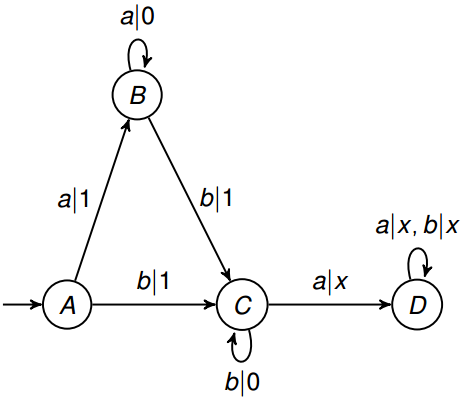
\includegraphics[scale=0.6]{images/MealyBsp.png}
\end{frame}

\begin{frame}{Mealy-Automat}
	\includegraphics[scale=0.25]{images/MealyEnd.png}
\end{frame}

\begin{frame}{Mealy-Automat}
	\includegraphics[scale=0.25]{images/MealyEndKonkat.png}
\end{frame}

\begin{frame}{Mealy-Automat}
	\includegraphics[scale=0.25]{images/MealyOut.png}
\end{frame}

\begin{frame}{Mealy-Automat}
	\includegraphics[scale=0.25]{images/MealyOutKonkat.png}
\end{frame}

\begin{frame}{Beispiel Mealy-Automat}
	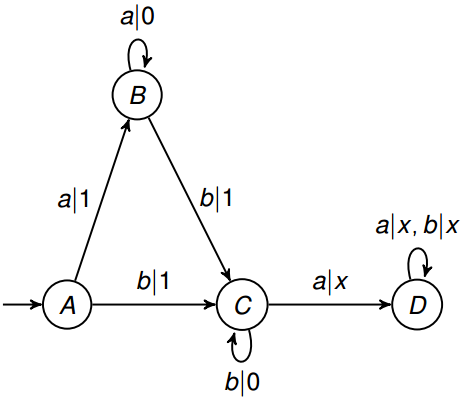
\includegraphics[scale=0.5]{images/MealyBsp.png}
	%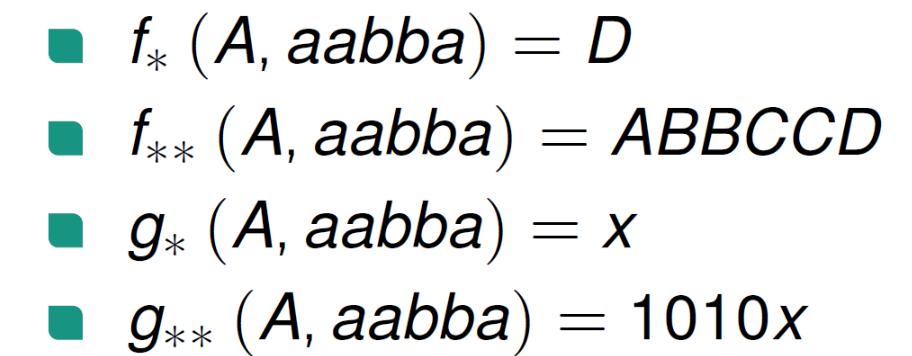
\includegraphics[scale=0.25]{images/MealyBspFunk.png}
	\begin{itemize}
		\item<1|only@1>[] {
			\begin{itemize}
				\item \(f_* (A, aabba) = D\)
				\item \(f_{**} (A, aabba) = ABBCCD\)
				\item \(g_* (A, aabba) = x\)
				\item \(g_{**} (A, aabba) = 1010x\)		
			\end{itemize}
		}
		\item<2-3|only@2-3>[] {
			\begin{itemize}
				\item[] Für welche \(w \in X^*\) gilt \(f_* (A, w) \neq D\)? \pause \pause
				\item[] Für genau alle \(w \in \{a\}^* \{b\}^*\).
			\end{itemize}
		}
		\item<4-5|only@4-5>[] {
			\begin{itemize}
				\item[] Für welche \(w \in X^*\) gilt \(g_* (A, w) = 0\)? \pause \pause
				\item[] Für genau alle \(w \in \{a\}^* \cdot \{b\} \cdot \{b\}^+ \cup \{a\} \cdot \{a\}^+\).
			\end{itemize}
		}
	\end{itemize}
\end{frame}

\subsection{Moore-Automat}

\begin{frame}{Moore-Automat}
	\begin{block}{Moore-Automat}
		Ein Moore-Automat ist ein Tupel $A = (Z, z_0, X, f, Y, h)$ mit...
		\begin{itemize}
			\item $Z$ endliche Zustandsmenge 
			\item $z_0 \in Z$ Anfangszustand 
			\item $X$ Eingabealphabet 
			\item $f: Z \times X \rightarrow Z$ Zustandsübergangsfunktion 
			\item $Y$ Ausgabealphabet 
			\pitem[$\rightarrow$] \textcolor{red}{Bis hierhin alles wie bei Mealy!}
			\pitem $h: Z \rightarrow Y^*$ Ausgabefunktion 
		\end{itemize}
	\end{block}

	\pause

	\begin{itemize}
		\pitem Zustände $\rightarrow$ Knoten
		\pitem Startzustand $\rightarrow$ Pfeil an diesen Knoten (nicht vergessen!)
		\pitem Zustandsüberführungsfunktion $\rightarrow$ Kanten mit Beschriftung \(w \in X\)
		\pitem Ausgabefunktion $\rightarrow$ zusätzliche Knotenbeschriftung \(w \in Y^*\)
	\end{itemize}
\end{frame}

\begin{frame}{Funktionen}
	\begin{itemize}
		\item \(f_*\) und \(f_{**}\) wie beim Mealy-Automaten
		\item \(g_* := h \circ f_*\)
		\item \(g_{**} := h_{**} \circ f_{**}\)
		Dabei bezeichnet \(h_{**}\) den durch \(h\) induzierten Homomorphismus.
	\end{itemize}
\end{frame}

\begin{frame}{Beispiel}
	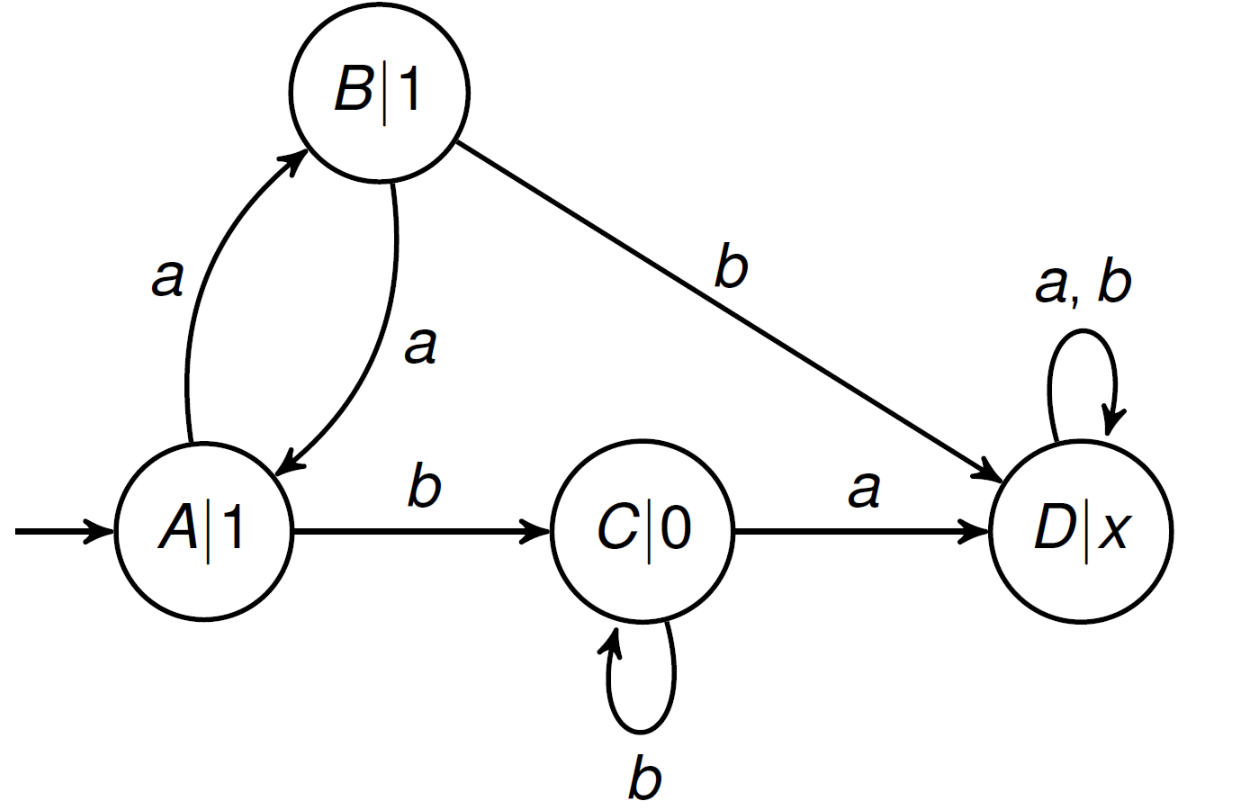
\includegraphics[scale=0.3]{images/Moore.png}
	\begin{itemize}
		\item<1|only@1>[] {
			\begin{itemize}
				\item \(f_* (A, aabba) = D\)
				\item \(f_{**} (A, aabba) = ABACCD\)
				\item \(g_* (A, aabba) = x\)
				\item \(g_{**} (A, aabba) = 11100x\)		
			\end{itemize}
		}
		\item<2-3|only@2-3>[] {
			\begin{itemize}
				\item[] Wann gilt \(g_* (A, w) = 0\)? \pause \pause
				\item[] Genau dann, wenn \(w \in \{aa\}^* \{b\}^+\).
			\end{itemize}
		}
	\end{itemize}
\end{frame}

\begin{frame}{Umwandlung}
	\textbf{Bemerkung}\\
	Für jeden Mealy-Automaten kann man einen Moore-Automaten konstruieren, der genau die gleiche Aufgabe erfüllt, und umgekehrt.
\end{frame}

%Mal selber ausprobieren lassen
\begin{frame}{Umwandlung Mealy- in Moore-Automat}
	Links ein Mealy-, rechts ein Moore-Automat
	
	
	\begin{figure}[!tbp]
		\centering
		\begin{minipage}[b]{0.4\textwidth}
			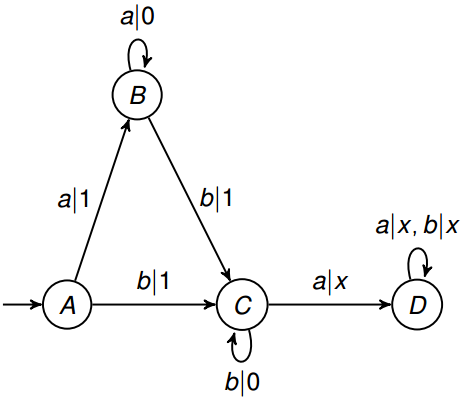
\includegraphics[width=\textwidth]{images/MealyBsp.png}
			\caption{Mealy}
		\end{minipage}
		\hfill
		\pause
		\begin{minipage}[b]{0.4\textwidth}
			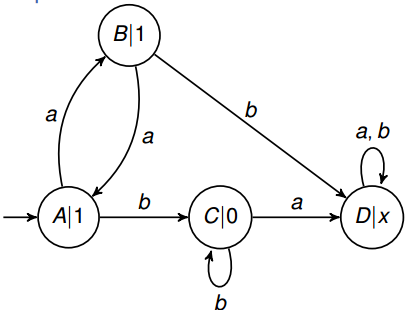
\includegraphics[width=\textwidth]{images/MooreBsp.png}
			\caption{Moore}
		\end{minipage}
	\end{figure}

\end{frame}

\subsection{Endliche Akzeptoren}
\begin{frame}{Endliche Akzeptoren}
	\begin{itemize}
		\pitem Sonderfall von Moore-Automaten
		\pitem Bei einem Akzeptor will man nur wissen, ob die Eingabe akzeptiert wurde oder nicht (also reicht ein Bit als Ausgabealphabet)
		\pitem Statt der Ausgabefunktion $h$ schreibt man einfach die Menge der akzeptierenden Zustände $F \subseteq Z$ auf
		\pitem Zustände, die nicht akzeptieren, heißen ablehnend
		\pitem Im Graphen werden akzeptierende Zustände einfach mit einem doppelten Kringel gekennzeichnet 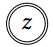
\includegraphics[scale=0.6]{images/Doppelkringel.png}
	\end{itemize}
\end{frame}

\begin{frame}{Akzeptierte Wörter und Sprachen}
	
	\begin{block}{Akzeptierte Wörter}
		Ein Wort $w \in X^*$ wird vom endlichen Akzeptor akzeptiert, wenn man ausgehend vom Anfangszustand bei Eingabe von w in einem akzeptierenden Zustand endet.
	\end{block}

	\pause
	
	\textbf{Bemerkung}\\
	\begin{itemize}
		\item Wird ein Wort nicht akzeptiert, dann wurde es abgelehnt
	\end{itemize}

	\pause
	
	\begin{block}{Akzeptierte formale Sprache}
		Die von einem Akzeptor $A$ akzeptierte formale Sprache $L(A)$ ist die Menge aller von ihm akzeptierten Wörter.
	\end{block}
\end{frame}

\begin{frame}{Endliche Akzeptoren}
	\begin{taskblock}{Aufgabe zu endlichen Akzeptoren}
		Konstruiere einen endlichen Akzeptor, der die Sprache $L_1(A) = \{w \in \{a,b\}^* : (N_a(w) \geq 3 \land N_b(w) \geq(2)\}$ erkennt.
	\end{taskblock}
	
	\pause
	\textbf{Lösung}\\
	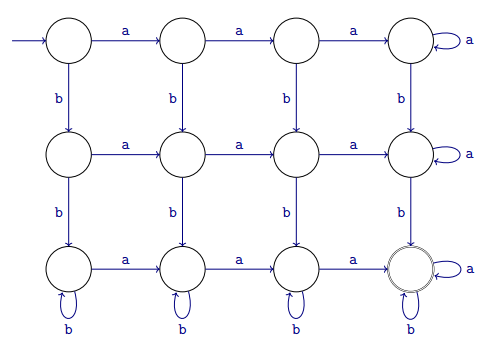
\includegraphics[scale=0.6]{images/AufgAkzeptor2.png}
\end{frame}
		
		

\begin{frame}{Endliche Akzeptoren}
	\begin{taskblock}{Aufgabe zu endlichen Akzeptoren}
		Konstruiere einen endlichen Akzeptor, der die Sprache $L_2(A) = \{w_1 ababb w_2| w_1, w_2 \in \{a,b\}^*\}$ erkennt.
	\end{taskblock}
	
	\pause
	\textbf{Lösung}\\
	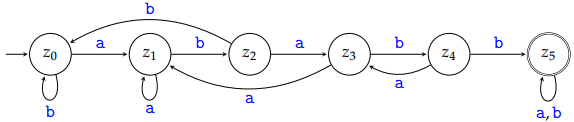
\includegraphics[scale=0.7]{images/AufgAkzeptor.png}\\
	\pause
	\begin{taskblock}{Aufgabe}
		Konstuiere einen endlichen Akzeptor der die Sprache $L_3 =\{w \in \{a,b\}^*| w \not \in L_2\}$ akzeptiert.
	\end{taskblock}
	\pause
	\textbf{Lösung} \\Ablehnende Zustände wereden zu akzeptierenden und andersrum.
\end{frame}		 

\begin{frame}{Endliche Akzeptoren}
	\begin{taskblock}{Aufgaben zu endlichen Akzeptoren}
		\begin{itemize}
			\item Gebe für den unten stehenden Automaten an, welche Sprache dieser akzeptiert.
			\item Gebe für die folgende Sprache über dem Alphabet $\{a,b\}$ einen endlichen Akzeptor an:
			$L = \{w \in \Sigma^* | N_a(w) \text{ mod } 3 > N_b(w) \text{ mod } 2\}$
		\end{itemize}
	\end{taskblock}

	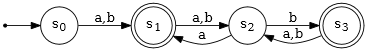
\includegraphics[scale=0.7]{images/AufgAkzeptor1.png}
\end{frame}

\begin{frame}{Lösungen}	
	\textbf{Lösung 1}\\
	$L = \{w \in \Sigma^* | |w| \text{ mod } 2 = 1\}$ (Worte ungerader Länger)\\
	\pause
	\textbf{Lösung 2}\\
	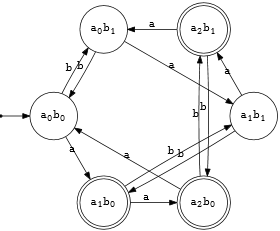
\includegraphics[scale=0.8]{images/LoesAkzeptor.png}
\end{frame}

\begin{frame}{Endliche Akzeptoren}
	Wann wird das leere Wort $\varepsilon$ von einem endlichen Akzeptor akzeptiert?\\
	\pause
	$\varepsilon \in L(A)$ gilt genau dann, wenn der Startzustand akzeptiert wird.
\end{frame}

\begin{frame}
Gibt es einen endlichen Akzeptor, der die Sprache $L_1=\{w \in \{1\}^*|$w ist Teilwort der Binärdarstellung von $ \pi\}$ erkennt \newline \pause
Gibt es einen endlichen Akzeptor, der die Sprache $L_2=\{0^k1^k|k\in \N_0\}$ erkennt
\end{frame}

\section{Turingmaschinen}

\begin{frame}{Turingmaschinen}
Was sind Turingmaschinen?

\begin{itemize}
	\pitem Sehr mächtige Erweiterung Automat
	\begin{itemize}
		\pitem Was heißt mächtig?
		\pitem Turingmaschinen können eine große Vielfalt von Problemen lösen, einschließlich vieler in GBI besprochener Probleme
	\end{itemize}
	\pitem Gesteuert durch einen endlichen Automaten\ip, aber mit einem \markBlue{unendlichen Arbeitsband} zum Zwischenspeichern von Informationen
	\pitem Besitzen einen Kopf um auf dem Band zu lesen und zu schreiben
	\pitem Turingmaschinen sind sozusagen genauso mächtig wie Computer
	\begin{itemize}
		\pitem können also benutzt werden, um für Probleme zu entscheiden, \markGreen{ob sie gelöst werden können oder nicht}
	\end{itemize}
\end{itemize}
\end{frame}

\begin{frame}{Definition von Turingmaschinen}
\begin{block}{Definition von Turingmaschinen}
Eine Turingmaschine $T = (Z, z_0, X, f, g, m)$ besteht aus:
\begin{itemize}
	\pitem $Z$ Zustandsmenge
	\pitem $z_0 \in Z$ Startzustand
	\pitem $X$ Bandalphabet
	\pitem $\Box$ Blanksymbol (sozusagen Markierung für Leerzeichen)
	\pitem $f: Z \times X \rightarrow Z$ partielle Zustandsübergangsfunktion
	\pitem $g: Z \times X \rightarrow X$ partielle Ausgabefunktion
	\pitem $m: Z \times X \rightarrow \{L, N, R\}$ partielle Bewegungsfunktion
\end{itemize}
\end{block}

Anmerkung: partielle Funktionen sind \markGreen{nicht linkstotal}, also manche Elemente des Definitionsbereichs werden nicht abgebildet.
\end{frame}

\begin{frame}{Beispiel einer Turingmaschine}
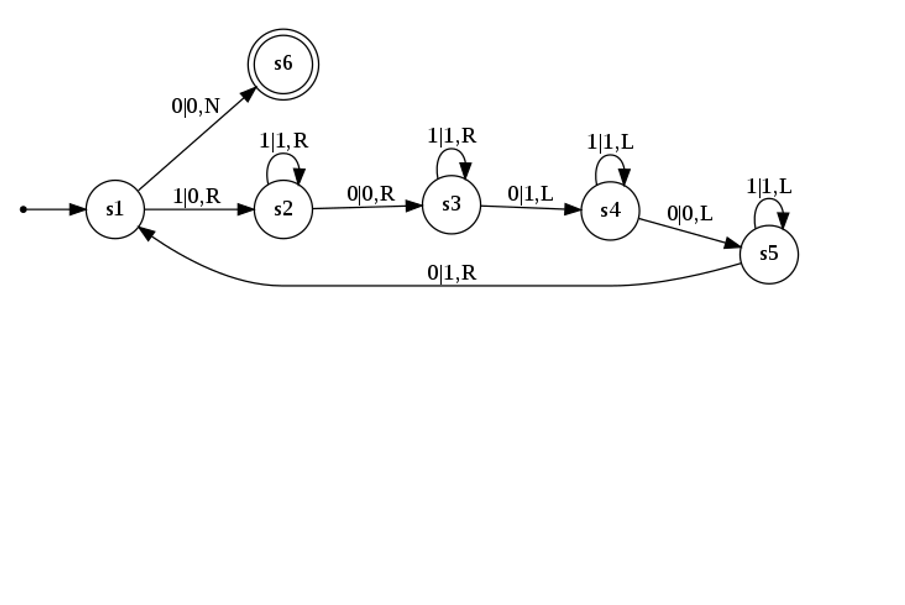
\includegraphics[scale=0.5]{images/turingexample_withoutannotations.png}
\end{frame}

\begin{frame}{Beispiel einer Turingmaschine}
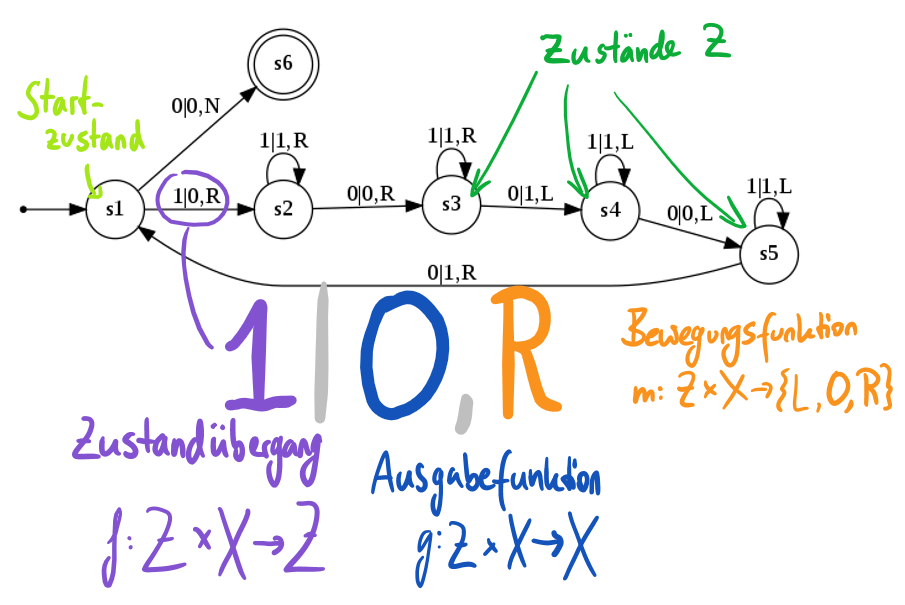
\includegraphics[scale=0.5]{images/turingexample_withannotations.png}
\end{frame}

\begin{frame}{Funktionen von Turingmaschinen}
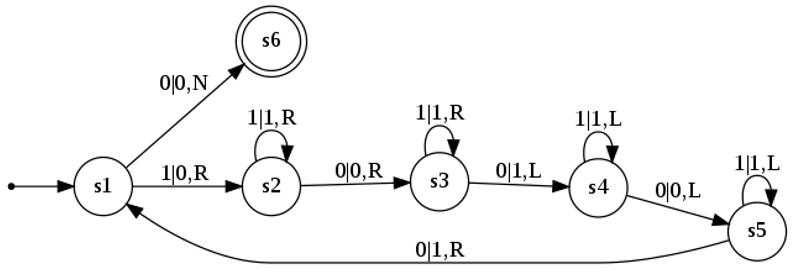
\includegraphics[scale=0.4]{images/turingexample_smallspacing.png}

Wie sehen die konkreten Abbildungsvorschriften der linken vier Pfeile aus?

\begin{columns}
\begin{column}{0.3\textwidth}

\vspace{.2cm}

% vielleicht an die tafel schreiben was die funktionen vom namen her machen (f: zustandsübergang), hat so nicht mehr auf die folie gepasst
\begin{itemize}
\item $f: Z \times X \rightarrow Z$
\item $g: Z \times X \rightarrow X$
\item $m: Z \times X \rightarrow \{L, N, R\}$
\end{itemize}
\end{column}

\begin{column}{0.7\textwidth}
\begin{tabular}{r || c | c | c}
& f & g & m\\\hline\hline

%erste Zeile als Beispiel
$0|0,N$ & $(s1, 0) \mapsto s6$ & $(s1, 0) \mapsto 0$ & $(s1, 0) \mapsto N$ \\\hline

\pause $1|0, R$ 
\pause & $(s1, 1) \mapsto s2$
\pause & $(s1, 1) \mapsto 0$
\pause & $(s1, 1) \mapsto R$ \\\hline

\pause $1|1, R$ 
\pause & $(s2, 1) \mapsto s2$
\pause & $(s2, 1) \mapsto 1$
\pause & $(s2, 1) \mapsto R$ \\\hline

\pause $0|0, R$ 
\pause & $(s2, 1) \mapsto s3$
\pause & $(s2, 1) \mapsto 0$
\pause & $(s2, 1) \mapsto R$ \\\hline

\end{tabular}
\end{column}
\end{columns}

\end{frame}


\begin{frame}{Das Band einer Turingmaschine}
\begin{itemize}
\pitem Unendliche Anreihung von Zeichen, die nach links und rechts unbegrenzt weiter geht

\p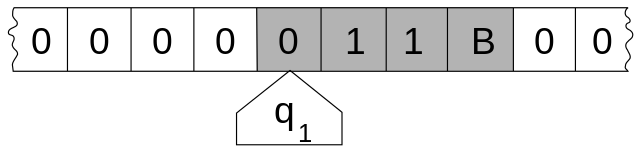
\includegraphics[scale=0.3]{images/turing_band.png}

\pitem Die Turingmaschine hat einen Kopf, mit dem sie das aktuelle Zeichen lesen oder überschreiben kann, oder kann ihn nach links oder rechts bewegen.

\pitem Das Band einer Turingmaschine wird benutzt als...
\begin{itemize}
\pitem Erhalten der Eingabe: \ip Bevor die Turingmaschine startet, steht das Eingabewort auf dem Band, der Kopf steht auf dem ersten Zeichen der Eingabe.
\pitem Rückgabe der Ausgabe: \ip Nach Beenden steht auf dem Band die Ausgabe (und der Kopf irgendwo).
\pitem Zwischenspeicher: \ip Die Turingmaschine kann überall Informationen zwischenspeichern, diese müssen von der TM am Ende aber gelöscht werden.
\end{itemize}
\end{itemize}
\end{frame}

% Am besten erst mal die aufgaben zusammen durchrechnen
\begin{frame}{Beispielabarbeitungen}
\begin{columns}
\begin{column}{0.5\textwidth}
\begin{taskblock}{Gemeinsame Übung}
Arbeite folgende Wörter mit der Turingmaschine ab:
\begin{itemize}
\item $0$
\item $1$
\item $11$
\item $111$
\end{itemize}
Was macht die Turingmaschine?
\end{taskblock}
\end{column}

\begin{column}{0.5\textwidth}
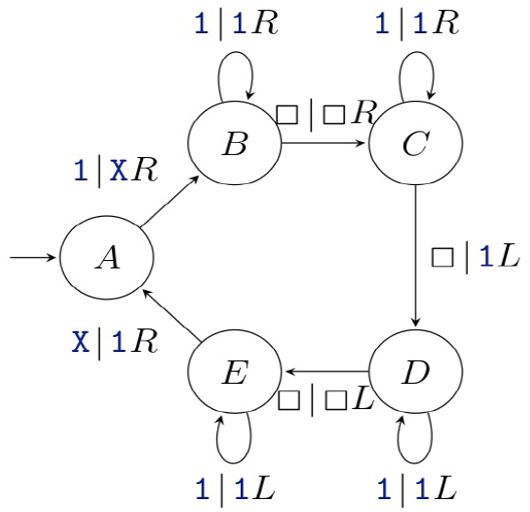
\includegraphics[scale=0.4]{images/turingmaschine_1k.png}
\end{column}
\end{columns}
\end{frame}


\begin{frame}
	
\includegraphics[width=\linewidth]{../images/thatsall.png}
\end{frame}


\end{document}